% -*- Mode:TeX -*-

%% IMPORTANT: The official thesis specifications are available at:
%%            http://libraries.mit.edu/archives/thesis-specs/
%%
%%            Please verify your thesis' formatting and copyright
%%            assignment before submission.  If you notice any
%%            discrepancies between these templates and the 
%%            MIT Libraries' specs, please let us know
%%            by e-mailing thesis@mit.edu

%% The documentclass options along with the pagestyle can be used to generate
%% a technical report, a draft copy, or a regular thesis.  You may need to
%% re-specify the pagestyle after you \include  cover.tex.  For more
%% information, see the first few lines of mitthesis.cls. 

%\documentclass[12pt,vi,twoside]{mitthesis}
%%
%%  If you want your thesis copyright to you instead of MIT, use the
%%  ``vi'' option, as above.
%%
%\documentclass[12pt,twoside,leftblank]{mitthesis}
%%
%% If you want blank pages before new chapters to be labelled ``This
%% Page Intentionally Left Blank'', use the ``leftblank'' option, as
%% above. 

\documentclass[12pt,twoside]{mitthesis}
\usepackage{lgrind}
\usepackage{graphicx}
\usepackage{draftwatermark}
\pagestyle{plain}
\widowpenalty10000
\clubpenalty10000

%% This bit allows you to either specify only the files which you wish to
%% process, or `all' to process all files which you \include.
%% Krishna Sethuraman (1990).

%%\typein [\files]{Enter file names to process, (chap1,chap2 ...), or `all' to
%%process all files:}
%%\def\all{all}
%%\ifx\files\all \typeout{Including all files.} \else \typeout{Including only \files.} \includeonly{\files} \fi



\begin{document}

% -*-latex-*-

\title{Scratching with All Your Fingers: Exploring Multi-touch Programming in Scratch}

\author{Christopher Graves}
\prevdegrees{ S.B., Massachusetts Institute of Technology (2013)}
% If you wish to list your previous degrees on the cover page, use the 
% previous degrees command:
%       \prevdegrees{A.A., Harvard University (1985)}
% You can use the \\ command to list multiple previous degrees
%       \prevdegrees{B.S., University of California (1978) \\
%                    S.M., Massachusetts Institute of Technology (1981)}
\department{Department of Electrical Engineering and Computer Science}

% If the thesis is for two degrees simultaneously, list them both
% separated by \and like this:
% \degree{Doctor of Philosophy \and Master of Science}
\degree{Master of Engineering in Electrical Engineering and Computer Science}

% As of the 2007-08 academic year, valid degree months are September, 
% February, or June.  The default is June.
\degreemonth{June}
\degreeyear{2014}
\thesisdate{May 23, 2014}

%% By default, the thesis will be copyrighted to MIT.  If you need to copyright
%% the thesis to yourself, just specify the `vi' documentclass option.  If for
%% some reason you want to exactly specify the copyright notice text, you can
%% use the \copyrightnoticetext command.  


% If there is more than one supervisor, use the \supervisor command
% once for each.
\supervisor{Mitchel Resnick}{LEGO Papert Professor of Learning Research, MIT Media Lab}

% This is the department committee chairman, not the thesis committee
% chairman.  You should replace this with your Department's Committee
% Chairman.
\chairman{Prof. Dennis M. Freeman}{Chairman, Masters of Engineering Thesis Committee}

% Make the titlepage based on the above information.  If you need
% something special and can't use the standard form, you can specify
% the exact text of the titlepage yourself.  Put it in a titlepage
% environment and leave blank lines where you want vertical space.
% The spaces will be adjusted to fill the entire page.  The dotted
% lines for the signatures are made with the \signature command.
\maketitle

% The abstractpage environment sets up everything on the page except
% the text itself.  The title and other header material are put at the
% top of the page, and the supervisors are listed at the bottom.  A
% new page is begun both before and after.  Of course, an abstract may
% be more than one page itself.  If you need more control over the
% format of the page, you can use the abstract environment, which puts
% the word "Abstract" at the beginning and single spaces its text.

%% You can either \input (*not* \include) your abstract file, or you can put
%% the text of the abstract directly between the \begin{abstractpage} and
%% \end{abstractpage} commands.

% First copy: start a new page, and save the page number.
\cleardoublepage
% Uncomment the next line if you do NOT want a page number on your
% abstract and acknowledgments pages.
% \pagestyle{empty}
\setcounter{savepage}{\thepage}
\begin{abstractpage}
% $Log: abstract.tex,v $
% Revision 1.1  93/05/14  14:56:25  starflt
% Initial revision
% 
% Revision 1.1  90/05/04  10:41:01  lwvanels
% Initial revision
% 
%
%% The text of your abstract and nothing else (other than comments) goes here.
%% It will be single-spaced and the rest of the text that is supposed to go on
%% the abstract page will be generated by the abstractpage environment.  This
%% file should be \input (not \include 'd) from cover.tex.

Since the introduction of the iPhone in 2007, many millions of people have used a multi-touch interface; but, due to the inaccessibility of most tablet software development kits, very few of these people have ever developed their own multi-touch interactions. This thesis discusses the challenges in developing a toolkit that allows novices to easily make simple touch-interactive projects, while simultaneously empowering experienced users to create complex, personalized multi-touch interactions. Three potential toolkit designs are presented and evaluated using the principle of ``low floors, wide walls, and high ceilings." The toolkits presented have been developed within the context of an upcoming tablet version of Scratch, which aims to allow users of all ages and educational backgrounds (but school-aged children in particular) to easily make and share their own stories, games, and animations on and for the tablet.
\end{abstractpage}

% Additional copy: start a new page, and reset the page number.  This way,
% the second copy of the abstract is not counted as separate pages.
% Uncomment the next 6 lines if you need two copies of the abstract
% page.
% \setcounter{page}{\thesavepage}
% \begin{abstractpage}
% % $Log: abstract.tex,v $
% Revision 1.1  93/05/14  14:56:25  starflt
% Initial revision
% 
% Revision 1.1  90/05/04  10:41:01  lwvanels
% Initial revision
% 
%
%% The text of your abstract and nothing else (other than comments) goes here.
%% It will be single-spaced and the rest of the text that is supposed to go on
%% the abstract page will be generated by the abstractpage environment.  This
%% file should be \input (not \include 'd) from cover.tex.

Since the introduction of the iPhone in 2007, many millions of people have used a multi-touch interface; but, due to the inaccessibility of most tablet software development kits, very few of these people have ever developed their own multi-touch interactions. This thesis discusses the challenges in developing a toolkit that allows novices to easily make simple touch-interactive projects, while simultaneously empowering experienced users to create complex, personalized multi-touch interactions. Three potential toolkit designs are presented and evaluated using the principle of ``low floors, wide walls, and high ceilings." The toolkits presented have been developed within the context of an upcoming tablet version of Scratch, which aims to allow users of all ages and educational backgrounds (but school-aged children in particular) to easily make and share their own stories, games, and animations on and for the tablet.
% \end{abstractpage}

\cleardoublepage

\section*{Acknowledgments}

This is the acknowledgments section.  You should replace this with your
own acknowledgments.

%%%%%%%%%%%%%%%%%%%%%%%%%%%%%%%%%%%%%%%%%%%%%%%%%%%%%%%%%%%%%%%%%%%%%%
% -*-latex-*-

\pagestyle{plain}
  % -*- Mode:TeX -*-
%% This file simply contains the commands that actually generate the table of
%% contents and lists of figures and tables.  You can omit any or all of
%% these files by simply taking out the appropriate command.  For more
%% information on these files, see appendix C.3.3 of the LaTeX manual. 
\tableofcontents
\newpage
\listoffigures


% This is an example of how you would use tgrind to include an example
% of source code; it is commented out in this template since the code
% example file does not exist.  To use it, you need to remove the '%' on the
% beginning of the line, and insert your own information in the call.
%
%\tagrind[htbp]{code/pmn.s.tex}{Post Multiply Normalization}{opt:pmn}

% This is an example of how you would use tgrind to include an example
% of source code; it is commented out in this template since the code
% example file does not exist.  To use it, you need to remove the '%' on the
% beginning of the line, and insert your own information in the call.
%
%\tgrind[htbp]{code/be.s.tex}{Block Exponent}{opt:be}




\chapter{Introduction} 
\section{Introduction to Scratch}
\subsection{Scratch Programming Environment}
\subsection{Introducing Tablet Scratch}
\section{Motivation}
\section{Touch Interactivity in Scratch}
\section{Thesis Overview}
hey hey hey \cite{1}



% This is an example of how you would use tgrind to include an example
% of source code; it is commented out in this template since the code
% example file does not exist.  To use it, you need to remove the '%' on the
% beginning of the line, and insert your own information in the call.
%
%\tagrind[htbp]{code/pmn.s.tex}{Post Multiply Normalization}{opt:pmn}

% This is an example of how you would use tgrind to include an example
% of source code; it is commented out in this template since the code
% example file does not exist.  To use it, you need to remove the '%' on the
% beginning of the line, and insert your own information in the call.
%
%\tgrind[htbp]{code/be.s.tex}{Block Exponent}{opt:be}



\chapter{Background}


\section{Desired Design Principles}
\section{Related Work}
\subsection{Textual Programming Languages}
\subsection{Graphical Programming Languages}
hey hey hey \cite{1}



\chapter{Case Projects}
It would be impossible to properly analyze the merits and faults of a variety of multi-touch interaction set designs without first considering a few of the most typical, potential use cases. In this chapter, I will present six project ideas that are representative of the kinds of projects that Tablet Scratchers of varying experience levels are likely to want to create. These six project ideas can be best thought of as three iterations of two basic projects: a Pong-style project and a finger-painting project. The three iterations are increasing in complexity and represent desirable projects for Scratchers at three different experience levels. I categorize the three iterations as \emph{low floor cases}, \emph{middle height cases}, and \emph{high ceiling cases}. The low floor cases represent simple, basic projects that even novice Scratchers should be able to intuitively create with little or no prior experience. Meanwhile, the middle height cases represent slightly more complicated additions that ought to be implementable by a Scratcher with significant experience. Finally, the high ceiling cases represent augmentations that an expert Scratcher might aspire to make. Together, these projects will serve as benchmarks for which I evaluate the multi-touch interaction set designs that I will present and analyze in the following three chapters.

\subsubsection{Introduction to Pong}
Designed by Allan Alcorn in 1972, Pong is widely considered to be the first culturally significant video game. Although rather simple in its original incarnation, many more complex variations have since been created.  In fact, Pong-style games are quite popular within the Desktop Scratch community, as evidenced by the thousands of variants that Scratchers have created and shared. Pong is a particularly fitting project to demonstrate the floors and ceilings of the multi-touch interaction set designs, since Pong projects can begin with very simple touch interactions that later become complex through the addition of more users and new actions.

\subsubsection{Introduction to Finger Painting}
Since the early 1900s, children all over the world have been expressing themselves through the art of finger painting. For many, painting with one's fingers is a calming, liberating experience. Due to their capacity for touch interactivity, tablet computers naturally lend themselves to being a means for finger painting, albeit cleaner and less textured. Like Pong, finger painting is another project that will help with presenting the floors and ceilings of the multi-touch interaction set designs. Although implementing painting for just one finger at a time is rather simple, the complexity increases dramatically as support for more fingers is added.

\section{Low Floor Cases}
It is worth restating that it is of paramount importance that the multi-touch interaction set be designed with a low floor in mind. Novice Tablet Scratchers must be able to easily figure out how to use the multi-touch interaction set to create simple projects that are responsive to touch. If beginners are able to create simple touch interactions without much difficulty, their early success will encourage them to augment their touch interactions and continue tinkering with their projects. Otherwise, if the process of creating simple touch-interactive projects is painful, many beginners will become frustrated and will forgo improving their projects. Here I specify two examples of basic projects that new Scratchers should be able to create without much assistance or hardship.

\subsection{Basic One-Player Pong}
The simplest form of Pong consists of a single paddle and a ball, which moves around the \emph{stage} (i.e., the background of a Scratch project) at a constant speed, rebounding whenever it hits either the paddle or a wall (Figure \ref{OnePlayerPong}). The paddle has a fixed y-coordinate (and thus cannot be moved up or down), but can be moved left and right. To begin any Pong project, one must first implement this basic functionality.

\begin{figure}
\centering
\includegraphics[width=0.6\textwidth]{images/OnePlayerPong.PNG}
\caption[One-Player Pong Screenshot]
{Here is a screenshot from a one-player Pong game.}
\label{OnePlayerPong}
\end{figure}

This single-player form of Pong has for a long time been one of the example starter projects in Desktop Scratch. In the starter project, the x-coordinate of the paddle is simply mapped to that of the mouse cursor. Therefore, users control the paddle by moving the mouse left and right. Note that in this case, the mouse controls the movement of the paddle regardless of whether or not the mouse cursor is hovering over the paddle. Unfortunately, we cannot use this control scheme for a Tablet Scratch project, since tablets do not have mice.

For this case project, I will specify an analogous touch control scheme for tablets. In the Tablet Scratch equivalent of this starter project, the paddle's x-coordinate will begin at an arbitrary default state. When a user touches the project, the paddle's x-coordinate will follow the x-coordinate of the user's touch. After the touch is lifted, the paddle's x-coordinate can either remain where it is or return to the arbitrary default state. 

The purpose of this case project is to test how easily novice Scratchers can create a single-finger touch interaction that relies on extracting coordinate information from a touch (in this case the x-coordinate) using the various multi-touch interaction sets. As a result, it will be assumed for this project that the user never presses two or more fingers on the tablet at the same time and I will leave it unspecified how the implementations of this project should handle such simultaneous touches.

\subsection{One-Finger Painting}
In the same way that one-player Pong is the simplest form of interactive Pong, a one-finger painting project is the most basic form of a finger-painting application. At its simplest, a one-finger painting application starts with a blank stage and paints an arbitrary color wherever the user touches the screen with one finger at a time (Figure \ref{OneFingerPainting}). Again, it will be assumed for this project that the user will not touch the screen with more than one finger at a time, so I will leave it unspecified how implementations should handle cases when the assumption is broken.

\begin{figure}
\centering
\includegraphics[width=0.6\textwidth]{images/OneFingerPainting.PNG}
\caption[One-Finger Painting Screenshot]
{Here is a sample painting made using a one-finger painting project.}
\label{OneFingerPainting}
\end{figure}

In Desktop Scratch, an analogue of this project can be created easily by using a \emph{pen}. As an homage to its predecessor, Logo, each sprite in Scratch carries a pen, which, when placed down, traces the movement of the sprite onto the stage. Consequently, a Scratcher would begin a ``mouse painting'' project in Desktop Scratch by first creating a \emph{paintbrush} sprite that follows the mouse cursor wherever it goes. Next, the Scratcher would program the paintbrush sprite's pen to start in the up position, but go down only when the mouse clicks down (meaning the pen only traces the movement of the mouse when the mouse is clicked down).

For the Tablet Scratch version of the project, the Scratcher would want the paintbrush sprite to initially have its pen up. Whenever a finger is pressed down, the sprite must be programmed to first move to the touch location, then put its pen down, and finally follow the touch until it is lifted. At the moment the touch is lifted, the sprite must be programmed to lift up its pen. Accordingly, the purpose of this case project is to demonstrate how easily a novice Scratcher can code a sprite to follow a touch and react to when the touch begins and ends.
 
At its core, this project is a simple exercise of recognizing and handling when a single finger is pressed down, when it moves, and when it is lifted. This capability is the building block to coding virtually all single-finger touch interactions. Thus, an interaction set that allows novice Tablet Scratchers to easily figure out how to implement this case project would be quite powerful.

\section{Middle Height Cases}
As Tablet Scratchers gain experience, they will naturally want to augment their simpler projects to develop progressively more complex ones. In addition to being intrinsically rewarding, the process of building upon earlier projects is a fundamental part of constructionist learning. Therefore, the ideal multi-touch interaction set must be designed so that as Tablet Scratchers master the basics of simple touch interactions, they can continue playing and figure out how to make more complex ones. If, on the other hand, the multi-touch interaction set is designed such that touch interactions more complex than the low floor cases are terribly difficult to achieve, then Tablet Scratchers would be stuck developing simple touch interactions and thus robbed of a learning opportunity. Here I present two natural augmentations an experienced Tablet Scratcher might want (and should be able) to add to the two previously described low floor cases. 

\subsection{Basic Two-Player Pong}
After a Tablet Scratcher successfully creates a simple one-player Pong project, the logical next step is to add a second player. For this case project, we again have a ball which moves around the stage with a constant speed, rebounding when it either hits a wall or a paddle. However, instead of one paddle with a fixed y-coordinate that moves only left and right, there are now, on either side of the stage, two paddles with fixed x-coordinates that move only up and down (Figure \ref{TwoPlayerPong}). Note that unlike in the one-player Pong project, this interaction cannot be developed in Desktop Scratch due to being limited to a single mouse.

\begin{figure}
\centering
\includegraphics[width=0.6\textwidth]{images/TwoPlayerPong.PNG}
\caption[Two-Player Pong Screenshot]
{Here is a screenshot from a two-player Pong game.}
\label{TwoPlayerPong}
\end{figure}

Clearly the controls from the one-player Pong project will not work in this case, because there could only be one touch at a time and that touch would control both paddles. For this case, I will assume that the paddles only follow the y-coordinate of a touch if the location of the touch is within a defined control range of the paddle and that the control range is small enough that no touch can simultaneously control both paddles. To make things simpler, it will be assumed that there are never more than two simultaneous touches and there is at most one touch at a time within either paddle's control range. 

The purpose of this case project is to compare the relative ease of using the various multi-touch interaction set designs to develop projects that require multiple sprites to respond to the touches that are closest to them. Without this functionality, many (even simple) multi-finger interactions will be impossible to develop. Although the capability for sprites to respond to all touches on the screen is obviously more powerful, an extensive range of the most common multi-touch interactions can be developed when the sprites' ability to respond to touches is limited to the ones that are closest to them.

\subsection{Two-Finger Painting}
Similar to how two-player Pong is the natural next step after one-player Pong, two-finger painting is the natural next step after one-finger painting. In two-finger painting, the user is able to draw on the stage with two fingers simultaneously instead of being limited to just one finger at a time (Figure \ref{TwoFingerPainting}). Again for simplicity, it will be assumed that the user never has more than two fingers simultaneously pressed on the tablet. Also note that, again, this kind of interaction cannot be developed for a single mouse in Desktop Scratch.

\begin{figure}
\centering
\includegraphics[width=0.6\textwidth]{images/TwoFingerPainting.PNG}
\caption[Two-Finger Painting Screenshot]
{Here is a sample painting made using a two-finger painting project.}
\label{TwoFingerPainting}
\end{figure}

This appended functionality adds a significant amount of complexity to the project. Now instead of having just one paintbrush sprite, there necessarily must be two paintbrush sprites to follow the up to two fingers pressed on the tablet. Moreover, when two fingers are being pressed at the same time, these two paintbrush sprites must be able to distribute themselves amongst the fingers, so that both fingers have a following paintbrush sprite. 

In contrast to the two-player Pong game, it is not enough in this project for the paintbrush sprites to simply follow the closest touch. If the paintbrush sprites were to do so, they would be prone to end up following the same finger, leaving the other finger without a paintbrush. There are many potential projects where it is necessary for sprites to distribute themselves among touches. Programming sprites to always follow separate fingers is a challenge, so the purpose of this project is to help distinguish which of the multi-touch interaction set designs make it easier.  

\section{High Ceiling Cases}
While Scratch's mission prioritizes having a low floor and wide walls, its high ceiling has been a major factor in its success. There are certain complex tasks, such as creating 3D graphics and online multiplayer capabilities, that are particularly difficult to develop in Scratch, but are possible to implement. Every day a few expert Scratchers implement and share projects that continue to push the bounds of what is possible to create in Scratch. Not only do the expert Scratchers gain a valuable learning experience by coding these challenging projects, but by sharing them with the community they inspire and educate Scratch beginners. By playing with the high ceiling projects and looking at how they were executed, less experienced Scratchers are motivated to continue challenging themselves and exploring what is possible. Thus, while complex multi-touch interactions might not necessarily be easy to program in Tablet Scratch, they should at least be possible to develop. Here I present two projects which feature advanced augmentations to the middle height case projects.

\subsection{Advanced Two-Player Pong}
While a basic two-player Pong game can be fun to play for a while, it is quite simple and eventually gets boring. The ball moves at a constant speed and players are limited to just moving their paddle up and down. In an attempt to make the game more interesting, an expert Scratcher might try adding a \emph{bump} action. A bump action causes the paddle to jut forward towards the opponent for a half-second before returning to its previously fixed x-coordinate. If the paddle hits the ball when it is in the process of a bump, the ball's speed increases by a constant factor. The bump action adds a little more skill and excitement to the basic two-player Pong project, but the question that remains is how will users instigate a bump action.

For this case project, a player will bump their paddle each time a second touch is pressed within a paddle's control range while there is already a touch there. More simply put, albeit slightly less rigorously, a bump happens whenever a user already using one finger to move the paddle presses their second finger close to the paddle.

At the core of this interaction is the capacity for sprites to recognize and handle not only the touch closest to them, but also all subsequent nearby touches. Although this interaction feels natural for this particular project case, it is very specific and unconventional. The ability to design and implement complex, multi-touch gestures adds a powerful means of personalizing Tablet Scratch projects. Hence, the ideal multi-touch interaction set design will make it possible to develop complex multi-touch controls like the one exhibited in this project.

\subsection{Ten-Finger Painting}
The next step for the finger-painting project after adding support for a second finger, is to add support for even more fingers. Since many Android devices can recognize up to ten simultaneous touches (not to mention that only a few people have more than ten fingers), this case project will be a finger painting application that supports up to ten simultaneous finger touches (Figure \ref{TenFingerPainting}). Many expert Tablet Scratchers will naturally try to make projects that allow users to deploy as many fingers as possible. Thus, the purpose of this case project is to test how well the multi-touch interaction sets make it possible to handle a large number of simultaneous touches. 

\begin{figure}
\centering
\includegraphics[width=0.6\textwidth]{images/TenFingerPainting.PNG}
\caption[Ten-Finger Painting Screenshot]
{Here is a sample painting made using a ten-finger painting project.}
\label{TenFingerPainting}
\end{figure}

Notice that the problems for this project are essentially the same as those regarding the two-finger painting project, but scaled by a factor of five. While the similarities might make this case project appear redundant, certain multi-touch interaction set designs make it easy to handle one or two fingers but terribly difficult to handle even a few more fingers. Meanwhile, other multi-touch interaction set designs make it a little challenging to handle one or two fingers, but not any more challenging to handle ten. I will discuss these trade-offs in the following three chapter as I introduce and analyze a selection of multi-touch interaction set designs.

%\chapter{Designs}
%
%There are so many degrees of freedom in specifying a multi-touch interaction set that it would be a herculean feat to even just enumerate all of the potential designs. Thus, in this chapter, I will specify and evaluate only the three most distinct and representative multi-touch interaction set designs, which I have designated as the \emph{Closest Finger Design},  the \emph{Relative Indexing Design}, and the \emph{Absolute Indexing Design}. While it is quite likely that the ``optimal'' multi-touch interaction set design will  be a composition of these three designs, I will present each of them undiluted and unmixed in order to best highlight their individual characteristics.
%
%The Closest Finger Design, can best be thought of as a direct analogue to the Desktop Scratch mouse interaction set. In this design, sprites can only listen to one touch at a time, namely the presently closest touch. As a result of this one touch restriction, the set of touch blocks in the Closest Finger Design closely resemble the set of mouse blocks in Desktop Scratch.
%
%In contrast to the first design, the Relative Indexing Design enables sprites to listen to each of the up-to-ten simultaneous touches. Touch inputs in this design are indexed relative to the other concurrent touches in order of initiation from $1$ to the number of current touches. Note that since touches are indexed relatively in this design, a touch's associated index can  be subject to change. For example, a touch that was the third oldest current touch (meaning it has an associated index of 3) can become the oldest current touch (meaning an associated index of 1) if the two oldest current touches are lifted.
%
%Finally, like the previous design, the  Absolute Indexing Design also enables sprites to listen to each of the up-to-ten simultaneous touches. However, touches in this design are indexed in order of initiation relative to all touches that have made since the inception of the project, as opposed to just the current touches. As a result, a touch's associated index can never change in the Absolute Indexing Design, because the $n$th touch pressed in the execution of a project will forever be the $n$th touch pressed.


\chapter{Closest Finger Design}

As mentioned previously, one reason why programming multi-touch interactions can be so difficult is that there can be up-to-ten simultaneous touches on the tablet at any given moment. Thus, multi-touch input handling in Tablet Scratch can be significantly simplified, by restricting each sprite to only being able to listen to the touch closest to itself. This particular restriction is the main premise behind the \emph{Closest Finger Design}, the first of the three multi-touch interaction set designs that I will be presenting.

In this chapter (as will be the pattern for the two subsequent chapters), I will first specify the Closest Finger Design interaction set. Then, I will evaluate the design on the three iterations of case projects that I described in the previous chapter. However, at the end of this particular chapter, I will also present a possible extension that provides additional functionality to the interaction set design, but at the cost of simplicity and understandability.

\section{Interaction Set Specification}

The Closest Finger Design can best be thought of as a direct analogue to the Desktop Scratch mouse interaction set. In this design, sprites can only listen to one touch at a time, namely the closest touch at the moment of evaluation. As a result of this one touch restriction, the set of touch blocks in the Closest Finger Design closely resemble the set of mouse blocks that appear in Desktop Scratch.

In fact, the Closest Finger Design has a corresponding touch block for every mouse-related block in Desktop Scratch. While, the mouse blocks in a Desktop Scratch script are influenced by the status of the lone mouse,  the Closest Finger Design blocks in a sprite's scripts are, in general, similarly influenced by the status of the touch that is currently closest to that particular Sprite. 

There are (as of now) eight blocks in Desktop Scratch that are related to mouse inputs: five function blocks, two command blocks, and a single hat block. I will  present all of these blocks while also introducing and specifying their Closest Finger Design block counterparts.

\begin{figure}
\centering
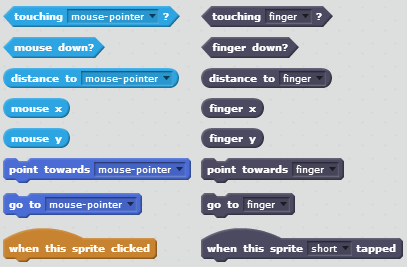
\includegraphics{images/Closest_Finger_Design_Block_Set.PNG}
\caption{Desktop Scratch's mouse interaction set with analogous Closest Finger Design blocks.}
\end{figure}

\subsection{Function Blocks}
The five mouse-related function blocks in Desktop Scratch are labeled ``touching mouse-pointer?", ``mouse down?", ``distance to mouse-pointer", ``mouse x", and ``mouse y". Following their namesakes, the ``touching mouse-pointer?" and ``mouse down?" blocks both produce Boolean values (e.g., \emph{true} or \emph{false}) corresponding to the current answer to their respective questions, while the ``distance to mouse-pointer", ``mouse x", and ``mouse y" blocks produce integer values (e.g., \emph{10}, \emph{-33}, \emph{147}, etc.) that similarly reflect their respective values. 

The first two equivalent Closest Finger Design function blocks, which I have labeled ``touching finger?" and ``finger pressed?", are relatively straight forward
\footnote{Note that these blocks reference ``fingers", but, in reality, most tablets cannot actually tell the difference between a touch coming from a finger or a touch coming from any other body part. However, for the sake of concreteness (and to avoid the potential confusion of a ``touch down" block), I have decided for blocks in the Closest Finger Design to refer to ``fingers" instead of ``touches".}.
As the name suggests, the ``touching finger?" block takes on a value of \emph{true} when a finger pressed on the tablet is touching the sprite using the block and a value of \emph{false} otherwise. Similarly, the ``finger pressed?" block takes on a value of \emph{true} when at least one finger is pressed on the stage and a value of \emph{false} when there are no touches.

The remaining three function blocks, labeled ``distance to finger", ``finger x", and ``finger y", are a little more difficult to articulate. In general, the ``distance to finger" block evaluates as the distance from the sprite to the touch that is currently closest to the sprite (i.e., the touch that has the shortest two dimensional distance to the center of the sprite with ties broken arbitrarily), while the ``finger x" and ``finger y" blocks represent the values of the latest x and y coordinates of that touch. When no fingers are currently being pressed on the tablet ``finger x" and ``finger y" will take the values corresponding to the location of last touch to have been made during the execution of the project. If the project just recently began and touches have yet to been made, ``finger x" and ``finger y" unfortunately must take on an arbitrary value. Since there is no ``null value" in Scratch and error messages are generally avoided, I have chosen for both ``finger x" and ``finger y" to evaluate to $0$ when no there are no prior touches. The ``distance to finger" block will always take the value of the distance between the current location of the sprite and the location with the coordinate values of ``finger x" and ``finger y".

\subsection{Command Blocks}
The two mouse-related command blocks in Desktop Scratch are the ``point towards mouse-pointer" and ``go to mouse-pointer" blocks, of which both when executed cause sprites to act as their names imply. Their equivalent Closest Finger Design blocks are similarly named ``point towards finger" and ``go to finger". Both of these blocks behave in a similar manner to their mouse counterparts, but focus on the location of the closest touch as opposed to that of the mouse.  

When there is at least one touch on the tablet, the location of interest for the blocks becomes that of the closest touch. Meanwhile, when no touches are currently present, the location of interest becomes the last location of the last touch. Finally, when no touches have been made during th execution of the project, the location of interest becomes the arbitrarily chosen coordinate of $\{0,0\}$.

To put it simply, executing the ``point towards finger" block cause sprites to point towards the location at the present coordinate values of ``finger x" and ``finger y". Similarly, executing the ``go to finger" block causes the sprite go to that same location. 

\subsection{Hat Block}
Finally, the sole hat block in Desktop Scratch's mouse interaction set is the ``when this sprite is clicked" block. When triggered, this hat block initiates the execution of its connected stack each time the sprite is clicked by the mouse. Here, a click is defined as pressing down on the mouse left button and quickly releasing. If the sprite is clicked a second time before the connected stack has finished its first execution, Scratch restarts the execution of the stack. Note that because of Scratch's thread-switching behavior, this can only happen when the stack contains loops or long ``wait blocks". 

The equivalent hat block for the Closest Finger Design is the ``when this sprite is tapped" block, which is triggered whenever a sprite is tapped. A sprite is said to be ``tapped" whenever a finger is pressed down on the sprite and quickly lifted. The ``when this sprite is tapped" block handles repeat triggerings in the same way as its mouse counterpart, i.e., by restarting the execution of the connected stack. Note that this hat block can be triggered by any touch, not just the closest touch, although in practice the triggering touch will almost always be the closest touch.

Since a variety of single-touch gestures, including swiping, long taps, and double taps, are common place in tablet applications, it may be beneficial to augment the ``when this sprite is tapped" block to support other common gestures. Adding support for more common single-touch gestures lowers the floors to implementing those interactions. However, this added support comes at the potential cost of narrowing the walls, since Scratchers might be encouraged to use the supported gestures instead of creating their own. Nevertheless, the interaction set is not fundamentally changed by adding support for other common single-touch gestures, so I will not be discussing in length which specific gestures are best to include.

\begin{figure}
\centering
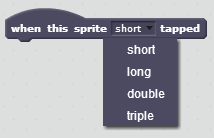
\includegraphics{images/When_This_Sprite_Is_Tapped.PNG}
\caption{The ``when this sprite is tapped" block expanded to demonstrate some of the simple gestures that could easily be supported.}
\end{figure}

\section{Evaluation}
Following intuition, the simplicity of the Closest Finger Design makes the simple low floor case projects easy to implement, but makes some of the harder case projects literally impossible to implement. While it is obvious that the Closest Finger Design simplifies the handling of single-touch inputs, surprisingly, a few common multi-touch interactions are also easy to implement using the design.

\subsection{Low Floor}
Due in part to the assumption of the existence of at most one touch on the tablet at a time, the Closest Finger Design excels with the low floor case projects. 

For example, the controls of the one-player Pong game can easily be implemented by constantly updating the x-coordinate of the paddle to the value of ``finger x". In the beginning of each game, the paddle's x-coordinate will first be mapped to $0$ (the arbitrary default value of ``finger x" before any touches have been made). After the first touch has been made, the paddle will follow the x-coordinate of the touching finger and will remain at its last location whenever the finger is lifted.

\begin{figure}
\centering
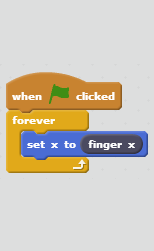
\includegraphics{images/OnePlayerPongCFD.PNG}
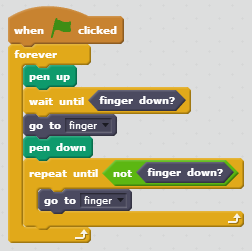
\includegraphics{images/OneFingerPaintingCFD.PNG}
\caption{On the left is an example of how the controls for one-player Pong could be implemented using the Closest Finger Design. On the right is an example script using the Closest Finger Design to program the paintbrush sprite in one-finger painting.}
\end{figure}

Implementing the controls for the one-finger painting project is a little more complicated, but is still straightforward and definitely within the capabilities of a novice Scratcher. Essentially, all the Scratcher must do is program the paint-brush to first wait for a touch to be made, then go to the touch's location and with its pen down continue following the touch until the finger is lifted. The Closest Finger Design, along with the additional framework blocks, makes programming this script almost as easy as just listing the instructions out in plain English (or any other of the sixty-six languages Scratch supports).

Recall that both of the low floor case projects were notable because they were the only two I presented that could be implemented in Desktop Scratch using mouse controls. As the result of the design's direct mapping with the Desktop Scratch mouse interaction set, many mouse-controlled Desktop Scratch projects can be directly translated into equivalent touch-controlled Tablet Scratch projects. This feature is of particular interest, because it may later become desirable for projects to be transferable between the desktop and tablet versions of Scratch.

\subsection{Middle Height}

Although both middle height case projects feature two sprites being controlled with to up-to-two simultaneous touches, one of the two project demonstrates the Closest Finger Design's greatest strength, while the other highlights its worst flaw. The two-player Pong game is well suited for this design, because the two paddles must each be programmed to follow the touch that is within their respective control ranges. On the other hand, the two paintbrush sprites in the two-finger painting project must be programmed to distribute themselves among up-to-two touches, a task that is all but impossible to program using the Closest Finger Design.

The controls for the basic two-player Pong game are extremely similar to that of the one-player Pong game when using the Closest Finger Design. In order to implement the interaction, each paddle can easily be programmed to constantly check to see if the value of ``distance to touch" is within the control range and, if that is the case, move the paddle vertically to the coordinate value ``finger y". 

\begin{figure}
\centering
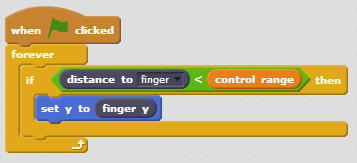
\includegraphics{images/BasicTwoPlayerPongCFD.PNG}
\caption{Here is an example script for the controlling the paddle in a basic two-player Pong game using the Closest Finger Design.}
\end{figure}

Even though each sprite can only listen to the touch nearest to themselves, many multi-touch interactions are still possible to implement. For example, it would also be simple to implement a multi-touch keyboard that allows multi-note chords to be played, just by programming each key to play its note when touched. The important factor in these implementable multi-touch interactions is that each sprite is only concerned with its closest touch, which makes the design's touch restriction advantageous rather than detrimental.

Despite the ease of implementing the basic two-player Pong game, it is terribly difficult to code the two-finger painting project using the Closest Finger Design. The main obstacle for this implementation is that each paintbrush sprite can only see the touch closest it to itself, even though it ,ay be necessary for one of the paintbrush sprites to follow the touch furthest from itself. 

One might think to first try to program the paintbrush to only follow its closest touch if the other paintbrush is not following it, but there are two significant problems with this approach. First, touches in the Closest Finger Design have no labels, so the only way to see if two sprites are listening to the same touch would be to compare their respective ``finger x" and ``finger y" values, which is an inelegant solution. Secondly, and more importantly, each paintbrush can only see the touch nearest to itself, so even if one paintbrush sprite realizes that its closest touch is already followed, it would not know where to go to find the other touch (if it even exists) and would thus have to travel around the stage looking for an unfollowed touch. While there may technically be an implementation of the two-finger painting project using the Closest Finger Design, that implementation would have to be so nonintuitive that it would not be worth considering for the purposes of this evaluation.

\subsection{High Ceiling}

Unfortunately, the simpleness of the Closest Finger Design makes the high ceiling projects essentially impossible to implement. Many complex multi-touch gestures simply cannot be implemented practically when each sprite can only listen to one touch. However, it is worth restating that many of the most popular tablet applications do not involve complex multi-touch gestures and those that do can often be redesigned to be functional with simpler controls.

Since the advanced two-player Pong game requires that each paddle simultaneously follow one touch while listening for subsequent touches that might initiate bump, it is strictly impossible to implement it exactly as specified using the Closest Finger Design. That being said, it would not be terribly difficult to make a functionally similar game with slightly more restricted controls using this interaction set. 

The implementation becomes significantly easier if the controls of the advanced two-player pong game are changed so that each paddle is moved by dragging and bumps are initiated by taps that are are close to, but not directly on the paddle. If this were the case, the paddle would simply be programmed to follow the closest touch only if the touch is within the bounds of the sprite (which can be checked using the ``touching finger?" block). To listen for bump initiating taps, a transparent crescent shaped bump detector sprite would then be created for each paddle. Both bump detectors would be programmed to follow their corresponding paddle. When a bump detector gets tapped, it would simply tell its corresponding paddle to initiate a bump.

\begin{figure}
\centering
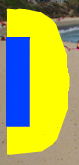
\includegraphics{images/LeftBumper.PNG}
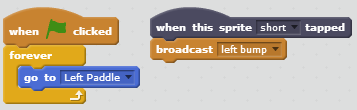
\includegraphics{images/BumperScript.PNG}
\caption{On the left is an example bump detector, colored yellow instead of transparent for visibility. On the right is the bumper detector script which programs the sprite to always follow the left paddle and to initiate a bump when tapped.}
\end{figure}

Unfortunately, the ten-finger painting project does not have a functionally equivalent alternative that is implementable with the Closest Finger Design. Since each paintbrush sprite can only see one touch and they have no practical way to distinguish which touches are not being followed, there does not exist a reasonable implementation for this project.

\section{Possible Extension}

Many of the limitations of the Closest Finger Design are the direct result of sprites only being able to listen to one touch at a time. While this restriction makes certain multi-touch interactions essentially impossible to program, it makes simple single-touch interactions very easy to program. Thus, the challenge in extending the Closest Finger Design to allow sprites to listen to multiple fingers lies in preserving the ease of programming simple touch controls.

\subsection{Specification}
The possible extension I will present is to add a new special hat block to the Closest Finger Design named ``when finger pressed". Note that the trigger for this block is different from that of the ``when this sprite is tapped" block. First, the ``when finger pressed" block is triggered by all touches, even ones whose locations are not on the sprite. Also, the ``when finger pressed" block is triggered whenever a finger first makes contact to tablet, as opposed to only being triggered by a quick tap. Furthermore, the ``when finger pressed"  block has two special properties which differentiate it from all other hat blocks.

The first special property is that the \emph{touch of interest} in the execution of a stack of blocks under a ``when finger pressed" block becomes the touch that triggered the execution of that hat block instead of just the closest touch. Before the addition of this extension, all of the five function blocks and two command blocks in the Closest Finger Design have always been solely focused on the sprite's presently closest touch. That is to say the touch of interest was always the In nearly all case with the extension, this is still true current closest touch. However, when these blocks are in a stack under a ``when finger pressed" hat, they correspond to the touch that triggered the hat as opposed to always corresponding to just the closest touch. Throughout the execution of the connected stack, the Closest Finger Design blocks will always refer to the touch that triggered the hat. If the touch that triggered the hat ends (i.e., is lifted) before the execution of the stack ends, the location of interest for all of the location related Closest Finger Design blocks becomes the last location of the triggering touch. 

This property allows sprites to listen to all touches as they are made, but only within the stack of blocks under a ``when finger pressed" block. Furthermore, the sprite loses access to the touch that triggered the ``when finger pressed" hat as soon as the connected stack has finished being executed (that is unless the touch is or becomes the sprite's closest touch). Thus, for some interactions, it will be beneficial to write the stack to continue running until the touch is lifted. However, this kind of script raises the question: what happens when a second touch is made when the stack under the ``when finger pressed" block is still executing from the first triggering? The answer to this question is the ``when finger pressed" block's second special property.

Instead of ignoring the second trigger or restarting the execution of its stack (as the other hats do), the ``when finger pressed" hat block essentially ``clones" its stack and executes it another in a thread. In each of these identical threads the touch of interest becomes the touch that triggered the making of the thread. Thus when three simultaneous touches are made, the stack connected to ``when finger pressed" block will execute three threads in parallel, each listening to a separate touch.
 
\subsection{Use Cases}

When augmented with the ``when finger pressed" hat block, the Closest Finger Design becomes powerful enough to implement the advanced two-player Pong game relatively easily . The paddles can use the ``when finger pressed" hat block to first find a touch to follow and then, when following the touch, listen for a bump initiating touch. The basic idea of the such a script is presented in Figure \ref{AdvancedTwoPlayerPongCFD}.

\begin{figure}
\centering
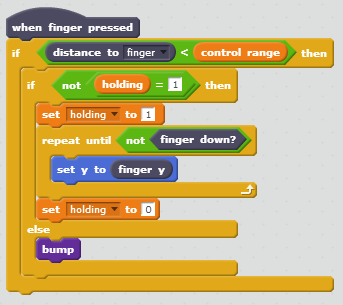
\includegraphics{images/AdvancedTwoPlayerPongCFD.PNG}
\caption{Example paddle script for advanced two-player pong using the ``when finger pressed" hat block.}
\label{AdvancedTwoPlayerPongCFD}
\end{figure}

The addition of the ``when finger pressed" block still does not make it possible to elegantly implement the multi-finger painting projects, but it does make it technically possible and significantly more practical to implement. Although all of the paintbrush sprites can listen to all of the touches with this augmentation, there still is no way to see which touches are already being followed other than the rudimentary method of checking if any of the paint brush sprites are already at the location of the touch in question. Thus, the multi-finger painting projects can be implemented by having each paintbrush use the ``when finger pressed" hat block to listen to all of the touches being made. If the paintbrush is not already following a touch, the paintbrush will follow the first incoming touch it encounters to the completion of touch if the touch is not already being followed. In figure I present the basic idea of this script.

\begin{figure}
\centering
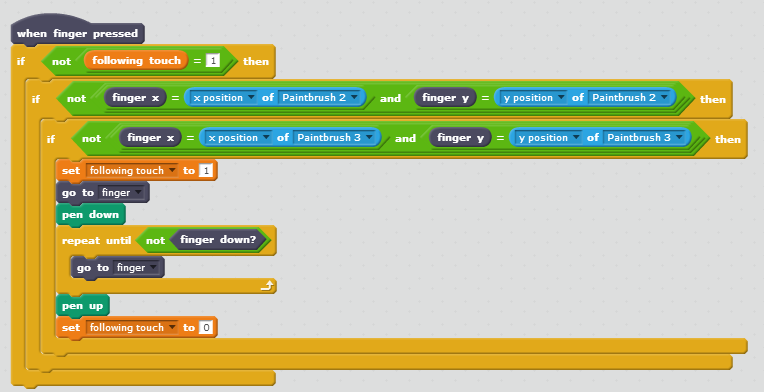
\includegraphics[width=1.0\textwidth]{images/MultiFingerPaintingCFD.PNG}
\caption{Example paintbrush script for three-finger painting using the ``when finger pressed" hat block. Note that more fingers can be supported by adding more paintbrush sprites and additional ``if checks".}
\label{MultiFingerPaintingCFD}
\end{figure}

\subsection{Potential Issues}
Although it is cause for concern that the ``when finger pressed" block's special influence on the touch blocks within its stack can be confusing to novice Scratchers, the main issues with the extension are a result of the block's thread-splitting feature.

One of Scratch's main design philosophies maintains that the execution of code should be visible. Since Scratch blocks are highlighted as they are executed, Scratchers can generally see in real time how their scripts are being executed. However, with the thread splitting, it is not clear how best to exhibit its execution when it is split into multiple threads. One idea would be to actually make copies of the stack as the threads are being created, but the tablet screen is so small that it could quickly become unwieldy when handling multiple simultaneous touches.

More importantly however, is the problem caused when a novice Scratcher innocently puts an infinite loop in the stack under a ``when finger pressed" hat block. In this case, a new, never-ending thread would be created at the initiation of every single touch. Since there is no bound on the total number of touches that can be made throughout the execution of a project, the number of threads that could be created is limitless. This potential for rapid thread propagation makes the project vulnerable to crashing from running out of computer resources without any indication to the novice Scratcher as to what is the cause. One possible solution would be to limit the number of threads to ten (since there can only be at most ten simultaneous touches), but the limit would be difficult to express visually and might restrict intentional use of the thread splitting feature.



\chapter{Relative Indexing Design}
While the Closest Finger Design does greatly simplify the task of handling up to ten simultaneous touches, it does so by avoidance. By restricting each sprite to only being able to listen to one touch at a time, the Closest Finger Design eludes having to handle ten touches within the same script. Even though this approach is reasonable, there are other potential strategies for simplification without such a restriction.

For example, one natural way to think about handling the up to ten simultaneous touches is to think of them as ten persistent touch-objects, among which all touch inputs are distributed. Since there can be at most ten simultaneous touch inputs, ten touch-objects are enough to handle all touch inputs made throughout the execution of any project. Each of these touch objects will be used to store the input values of the touch it is currently associated with, i.e. the x and y coordinates of the touch and whether the touch is being pressed on the tablet. The big question with such a design becomes: What is the best way to distribute the touch inputs amongst the ten touch-objects?

In this second multi-touch interaction set design, which I have named the \emph{Relative Indexing Design}, the persistent touch-objects are indexed $1$ through $10$ and represent the status of the touch inputs with matching indices. The touch inputs are indexed relative to the other concurrent touches in order of initiation from $1$ to the number of current touches. Since touches are (as the design's name implies) indexed relatively, a touch's associated index (and, thus, associated persistent touch-object) can  be subject to change. For example, a touch that was the third-oldest current touch (meaning it has an associated index of 3) can become the oldest current touch (meaning an associated index of 1) if the two older current touches are lifted. While this manner of indexing is intuitive, it has a few quirks that can lead to many unforeseen bugs in the development of seemingly simple projects.

In this chapter, I will first specify the Relative Indexing Design and then follow up by evaluating the design on the three iterations of case projects that I described in Chapter 3.

\section{Interaction Set Specification}

The Relative Indexing Design consists of nine touch blocks, only one of which is wholly original to this thesis: the ``number of fingers" block (Figure \ref{Number_Of_Fingers}). As the name implies, the ``number of fingers" block produces a value ranging from \emph{0} to \emph{10}, representing the number of fingers on the tablet at the time of evaluation. Since most tablets can only recognize up to ten simultaneous touches, the ``number of fingers" block will return the value of \emph{10} whenever there are 10 or more touches.

\begin{figure}
\centering

\includegraphics{images/Number_Of_Fingers.PNG}
\caption[The ``number of fingers" Block]{The ``number of fingers" block.}
\label{Number_Of_Fingers}
\end{figure}

The remaining eight touch blocks in the Relative Indexing Design are similar in appearance to the extended Closest Finger Design interaction set minus the ``when this sprite is tapped" block. The only difference is that each of the Relative Indexing Design blocks has an added numerical parameter (see left side of Figure \ref{Relative_Indexing_Design_Block_Set}). This parameter is used to select the index (ranging from 1 to 10) of the desired touch of interest.\footnote{Note that in these blocks I again use the term ``finger" instead of touch. Although this terminology could lead some novices into thinking that the touch indices correspond to particular fingers (e.g., finger 5 always refers to the user's left thumb), I believe it is still beneficial to use the concrete term ``finger," rather than the abstract term ``touch."}
The parameter is a drop-down menu with values ranging from 1 to 10, but it is also a slot that can be filled with a function block (see right side of Figure \ref{Relative_Indexing_Design_Block_Set}). If the inserted function block returns a value other than an integer between 1 and 10, the value gets defaulted to 1, so as to avoid throwing errors.

\begin{figure}
\centering
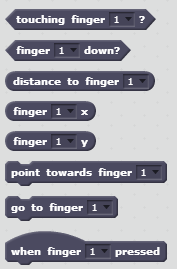
\includegraphics{images/Relative_Indexing_Design_Block_Set.PNG}
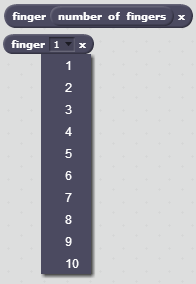
\includegraphics{images/Relative_Indexing_Design_Block_Dropdown_Show.PNG}
\caption[Remaining Eight Blocks in the Relative Indexing Design Interaction Set]{On the left are the remaining eight blocks in the Relative Indexing Design interaction set.  On the right there are two examples of the ``finger (\emph{index}) x" block: one with the drop-down menu opened and the other with an inserted function block.}
\label{Relative_Indexing_Design_Block_Set}
\end{figure}

Of these eight remaining touch blocks, only two, the ``finger (\emph{index}) down?" and ``when finger (\emph{index}) pressed" blocks, are not affected by the location of the touch inputs, so I will quickly explain them first. The ``finger (\emph{index}) down?" block is a simple Boolean function block that returns a value of \emph{true} if the touch with the index of (\emph{index}) is currently down and a value of \emph{false} otherwise. By the nature of relative indexing, this is the equivalent of determining whether
there are at least (\emph{index}) touches currently pressed on the tablet. As a result, the ``finger (\emph{index}) down?" block is redundant, since this value can be determined using the ``number of fingers" block along with some logic blocks. Even so, the ``finger (\emph{index}) down?" block is a worthwhile shortcut, because it can become tedious to determine the value repeatedly.

The ``when finger (\emph{index}) pressed" block is a simple trigger block that is closely related to the ``finger (\emph{index}) down?" function block. The ``when finger (\emph{index}) pressed" block is triggered at the moment the finger with the index of (\emph{index}) is pressed. In other words, the ``when finger (\emph{index}) pressed" block executes its connected stack at the moment the number of touches on the tablet increases from (\emph{index-1}) to (\emph{index}). Unlike its extended Closest Finger Design counterpart, which creates new threads for every triggering, the ``when finger (\emph{index}) pressed" block restarts the execution of its connected stack when it is triggered for a second time before finishing the first execution.

The final six blocks, ``touching finger (\emph{index})?", ``distance to finger (\emph{index})," ``point towards finger (\emph{index})," ``go to finger (\emph{index})," ``finger (\emph{index}) x," and ``finger (\emph{index}) y," behave the same as their Closest Finger Design counterparts except that their location of interest is the current location of the touch with the index of (\emph{index}) instead of the sprite's closest touch. When (\emph{index}) is less than or equal to the current number of touches (i.e., the ``finger (\emph{index}) down?" block evaluates to \emph{true}), the location touch with the index of (\emph{index}) is simply the location of the (\emph{index})th-longest-lasting touch currently on the tablet. Otherwise, when (\emph{index}) is greater than the current number of touches (i.e., the ``finger (\emph{index}) down?" block evaluates to \emph{false}), the location of the touch with the index of (\emph{index}) remains at its last location. Again, prior to all touches, the fingers of all indices have the arbitrary, default  location of $\{0,0\}$.

\section{Evaluation}

Due to the functionality of the Relative Indexing Design being fairly straightforward, many of the simpler multi-touch interactions can be implemented intuitively. However, as projects get more complicated, the limitations of the Relative Indexing Design become evident.

\subsection{Low Floor}
For projects that assume a maximum of one touch on the screen at a time, the  Relative Indexing Design has the capability to behave identically to the Closest Finger Design. When there is only one touch on the screen, that touch is every sprite's closest touch. Similarly, the relative index of the single touch will, by definition, always be 1. Thus, both the one-player Pong game and the one-finger painting project can be implemented using the Relative Indexing Design in essentially the same way as they were implemented in the Closest Finger Design in the previous chapter (Figure \ref{LowFloorRID}).

\begin{figure}
\centering
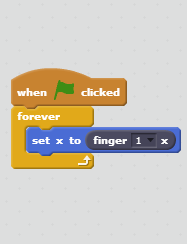
\includegraphics{images/OnePlayerPongRID.PNG}
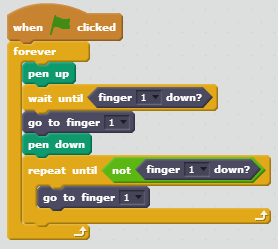
\includegraphics{images/OneFingerPaintingRID.PNG}
\caption[Sample Relative Indexing Design Scripts for Low Floor Case Projects]{On the left is the Relative Indexing Design script for the one-player Pong game paddle controls.  On the right is the script for one-finger painting.}
\label{LowFloorRID}
\end{figure}

Although  these low floor case projects can be implemented using the Relative Indexing Design as easily as with the Closest Finger Design, the latter does a slightly better job of lowering the floors. The parameter in the Relative Indexing Design blocks does not provide any added functionality for single-touch projects, so it can only contribute to potential confusion.

\subsection{Middle Height}

The middle height case projects are not particularly well suited for the Relative Indexing Design. To begin with, the Relative Indexing Design does not filter the touch inputs for the closest touch (unlike the Closest Finger Design). As a result, implementing the basic two-player Pong game is slightly more laborious, even though it is still a relatively straightforward process (Figure \ref{BasicTwoPlayerPongRID}). Since we have the assumption that there will be at most two simultaneous touches, both paddles only have to listen to the touches with indices 1 or 2. For each paddle, it does not matter whether a touch was the first or the second touch made. Thus, the paddle's script must forever repeat the process of checking both touches and follow the y-coordinate of the touch that is within the paddle's control range (if there is such a touch).

\begin{figure}
\centering
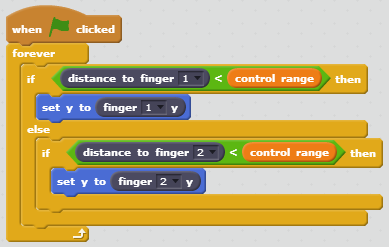
\includegraphics{images/BasicTwoPlayerPongRID.PNG}
\caption[Sample Relative Indexing Design Script for Basic Two-Player Pong]{Here is a sample script for controlling the paddle in a basic two-player Pong game using the Relative Indexing Design.}
\label{BasicTwoPlayerPongRID}
\end{figure}

This implementation is fairly easy to follow when presented, but has a few subtleties that can be tricky for Scratchers to figure out. For example, if a Scratcher is not careful, it is possible to fall victim to the bug of having the paddle stuck ``following" an already lifted touch. While these bugs can be tricky for beginners, they are relatively concrete as far as bugs go, so I am confident that Scratchers (especially with the help of the supportive Scratch community) will be able to overcome them and learn from them. 

Similarly, implementing the two-finger painting project using the Relative Indexing Design also has a few subtle pitfalls. However, unlike the case for the basic two-player Pong game, the bugs that arise when implementing the two-finger painting project are very difficult to overcome. Naive intuition would suggest that each paintbrush sprite wait for and subsequently follow a different indexed touch. In other words, one paint brush would follow the first touch when it occurs and the second paint brush would follow the second touch when it occurs (left side of Figure \ref{NaiveTwoFingerPaintingRID}).

\begin{figure}
\centering
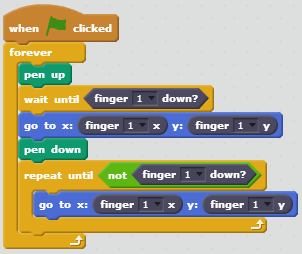
\includegraphics[width=0.415\textwidth]{images/NaiveTwoFingerPaintingRID.PNG}
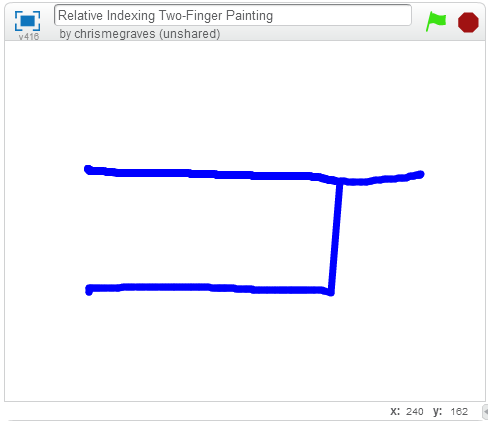
\includegraphics[width=0.4\textwidth]{images/IndexTransferLineBug.PNG}
\caption[Sample Naive Script for Two-Finger Painting Using the Relative Indexing Design ]{On the left is a sample naive paintbrush script using the Relative Indexing Design. On the right is the result of the bug caused by the touch index transferring.}
\label{NaiveTwoFingerPaintingRID}
\end{figure}

This control scheme works for the most part, but there is a pernicious bug for which there is no simple solution. The bug occurs when there are two touches simultaneously on the tablet, and the touch with index 1 (i.e., the first touch) is lifted before the touch with index 2 (i.e., the second touch). At this moment, the paintbrush following the second created touch stops following it, because ``finger (2) down?" would evaluate to \emph{false}. Also, the paintbrush following the first touch, would then start to follow the second touch, since its index changed from 2 to 1. This transfer is fine, but the problem is that the paintbrush following the first touch does not know to lift up its pen before starting to follow the second paintbrush, leading to an unintentional line in the user's painting (e.g., right side of Figure \ref{NaiveTwoFingerPaintingRID}). 

There are reasonable solutions (e.g., left side of Figure \ref{WaryTwoFingerPaintingRID}) to the bug that prevent the unintentional line from appearing, but they result in small gaps in the finger painting lines (e.g., right side of Figure \ref{WaryTwoFingerPaintingRID}). Furthermore, even these imperfect solutions pose a considerable challenge to experienced Scratchers. A ``perfect," practical implementation for multi-finger painting cannot be done using the Relative Indexing Design, because some data will be lost when the touch index transfers occur. This loss of data is due in part to the fact that there is no sure way to differentiate between two similar but importantly distinct events: the event in which the first touch is lifted before the second and the event in which the second touch is lifted before the first. That being said, reasonable assumptions can be made by comparing touch locations, as was the case for the Closest Finger Design. 

\begin{figure}
\centering
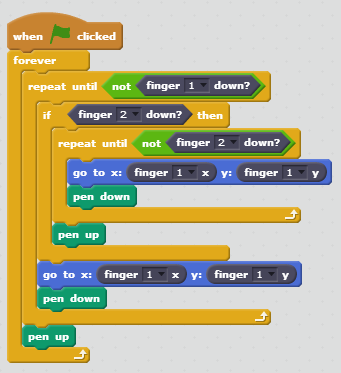
\includegraphics[width=0.4\textwidth]{images/WaryTwoFingerPaintingRID.PNG}
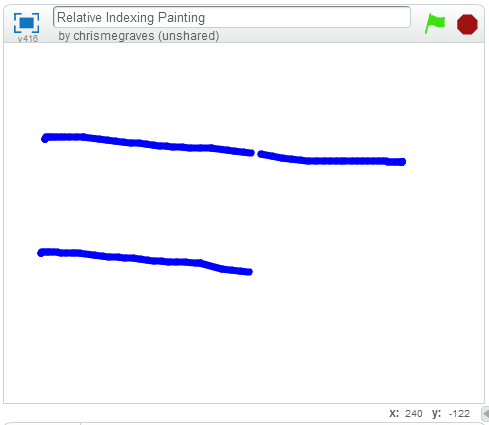
\includegraphics[width=0.5\textwidth]{images/IndexTransferGapBug.PNG}
\caption[Sample ``Wary" Script for Two-Finger Painting Using the Relative Indexing Design ]{On the left is a sample ``wary" script for the paintbrush using the Relative Indexing Design. On the right is the result of the bug that still exists in the ``wary" script.}
\label{WaryTwoFingerPaintingRID}
\end{figure}

\subsection{High Ceiling}

Since the Relative Indexing Design makes it impossible to practically implement a ``perfect" two-finger painting project, the same holds for the ten-finger painting project. Also, as the reader might imagine, the added logic needed to minimize (but not eliminate) the bugs in the two-finger project becomes much more convoluted when support for more fingers is added, because all touch index transfers must be accounted for. That being said, the level of complexity for the needed, additional logic is in line with the expected amount of difficulty for high ceiling projects. Although assembling the blocks would be tedious, the logic behind handling the transfers follows a pattern that can be repeated.

Similarly, the advanced two-player Pong game is quite difficult to implement using the Relative Indexing Design, but it can be done, and the amount of work and expertise needed is appropriate for a high ceiling project. Unlike the ten-finger painting project, however, the advanced two-player Pong game can be implemented exactly as specified with the Relative Indexing Design. The script for the advanced two-player Pong game paddle controls can be a little complicated (Figure \ref{AdvancedTwoPlayerPongRID}), but the logic is fairly straightforward. 

\begin{figure}
\centering
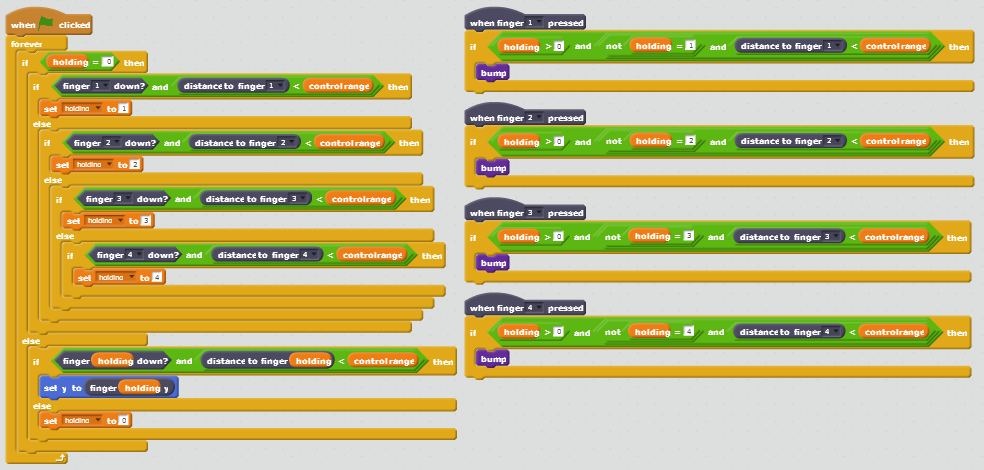
\includegraphics[width=1.0\textwidth]{images/AdvancedTwoPlayerPongRID.PNG}
\caption[Sample Relative Indexing Design Script for Advanced Two-Player Pong]{Here is a sample script for controlling the paddle in an advanced two-player Pong game using the Relative Indexing Design.}
\label{AdvancedTwoPlayerPongRID}
\end{figure}

The controls can be implemented using one ``forever loop" to control the movement and four ``when finger (\emph{index}) pressed" stacks to wait for bump-initiating taps. The ``forever loop" would first check if the paddle is currently following a finger. If the paddle is not following a finger, its script will query the touches with indices 1 through 4 (since we are assuming no more than four simultaneous touches) and decide to follow the first finger index it queries that is both down and within the paddle's control range. After deciding to follow a finger index, the paddle will follow that finger index until it is either lifted or moved out of range. 

The four ``when finger (\emph{index}) pressed" blocks will watch the finger indices 1 through 4. Their connected stacks will check for three criteria and, if they are met, will initiate a bump. The first criterion is that the paddle is currently following a touch. The second is that the touch being followed is not the touch that triggered the execution of the stack. Finally, the last criterion is that the touch that triggered the stack is within the paddle's control range.

As evidenced by the high ceiling case projects, the Relative Indexing Design does not make implementing complex projects particularly easy. However, the design does make their implementations possible (or at least almost possible, as is the case for the multi-finger painting projects). The intuitions for these implementations are almost always straightforward, but the actual assembly of the implementations can be tedious. Furthermore, there are subtle quirks with the Relative Indexing Design that are the basis for some tricky (albeit oftentimes surmountable) bugs.





\chapter{Absolute Indexing Design}

Without a doubt, the multi-finger painting case projects have proven to be the most troublesome to implement using both of the two previously presented designs. It is impossible to elegantly implement a multi-finger painting project using the Closest Finger Design, because the design does not offer a method to differentiate between individual touches other than through the comparison of touch locations. The Relative Indexing Design suffers from a similar inability. Although the Relative Indexing Design makes it easy to distinguish all of the present touches (using their relative indices), the design does not enable scripts to determine when touches switch indices. As a result, it is difficult to program paintbrushes to follow specific touches, since the touches' associated indices are subject to change. If every touch were given a unique index that it kept from its creation to its end (i.e., an ID number), then it would not be difficult to distribute touches amongst the paintbrush sprites so that every touch is followed by exactly one paintbrush.

This concept, assigning each created touch a unique, permanent  number, is the main premise behind the \emph{Absolute Indexing Design}, the third and final multi-interaction set design. Touches in the Absolute Indexing Design are indexed in order of initiation relative to all touches that have been made since the inception of the project. As a result, a touch's associated index can never change in the Absolute Indexing Design, because the $n$th touch pressed in the execution of a project will forever be the $n$th touch pressed.

While the Absolute Indexing Design can facilitate the implementation of certain complex multi-touch interactions, it can make implementing simpler single-touch interactions more difficult. In this chapter, I will again first specify the design and afterwards evaluate it using the three iterations of case projects described in Chapter 3.

\section{Interaction Set Specification}

The Absolute Indexing Design consists of nine blocks (Figure \ref{FamiliarAIDBlocks}), only two of which are wholly original. In contrast to the previous chapter, I will specify the familiar blocks before presenting the newer ones.

The seven familiar blocks in the Absolute Indexing Design each have counterparts in the Relative Indexing Design, but with two main differences. The first difference between these blocks and their Relative Indexing Design counterparts is that their parameters are text inputs rather than drop-down menus. Since the touch indices are not bounded by 10 in the Absolute Indexing Design, a drop-down menu would not make sense. Also, these parameters are best thought of as (\emph{ID})s instead of (\emph{index})es. The second difference is that the term ``finger" is replaced with ``touch" in the block labels. Although the use of the term ``finger" was not perfectly suitable in the Relative Indexing Design either, the term ``finger"  makes no sense at all when using absolute indexing. For example, the term ``finger (73)" implies that the user has at least 73 fingers, whereas ``touch (73)" accurately implies the 73rd touch pressed on the tablet.

Thus, the seven familiar blocks are named: ``touch (\emph{ID}) down?", ``touching touch (\emph{ID})?", ``distance to touch (\emph{ID})," ``point towards touch (\emph{ID})," ``go to touch (\emph{ID})," ``touch (\emph{ID}) x," and ``touch (\emph{ID}) y." Functionally, these seven Absolute Indexing Design blocks work in a manner similar to their Relative Indexing Design counterparts, just with different touch indexing. For example, the ``touch (\emph{ID}) down?" block reports the value of \emph{true} if the (\emph{ID})th touch in the project's execution  has been created and is still touching the tablet and otherwise reports the value of \emph{false}. Similarly, the remaining six familiar blocks all correspond to the location of the (\emph{ID})th touch in the project's execution. If the (\emph{ID})th touch has yet to be made, its location is considered to be $\{0,0\}$. Also, if the (\emph{ID})th touch has already been both made and lifted, its location is considered to be its last touched location. If the inserted value of (\emph{ID}) is anything other than a positive integer, the location of interest is always defaulted to $\{0,0\}$.

\begin{figure}
\centering
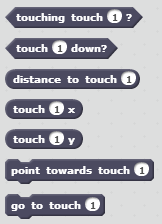
\includegraphics{images/FamiliarAIDBlocks.PNG}
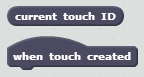
\includegraphics{images/NewAIDBlocks.PNG}
\caption[The Absolute Indexing Design Interaction Set]
{The seven familiar blocks in the Absolute Index Designs are on the left, while the two new blocks are on the right.}
\label{FamiliarAIDBlocks}
\end{figure}

Now that the familiar blocks have been specified, I will introduce the two original blocks. The first of the entirely new blocks is a function block, labeled ``current touch ID." Simply put, the ``current touch ID" block reports the unique ID of the most recently made touch. When touches have yet to be made, the ``current touch ID" block reports the value 0, since the first touch in the execution of a project has an ID of 1. An important aspect of the behavior of the ``current touch ID" is that it increases by at most 1 per execution iteration of the Scratch programming environment. In other words, if a loop in Scratch is constantly checking the value of the ``current touch ID" block at each iteration (without having inner loops or ``wait" blocks), the value will not jump from \emph{x} to \emph{x+2} without being valued as \emph{x+1} first, even if two touches are made simultaneously. Thus, it is possible to watch the ``current touch ID" block without having to worry about missing a touch.

The second new block is a trigger block labeled, ``when touch created." In many ways  the ``when touch created" block is analogous to the ``when finger pressed" block from the extended version of the Closest Finger Design and the ``when finger (\emph{index}) pressed" block from the Relative Indexing Design. However, its behavior is unique and important to the Absolute Indexing Design. Like the ``when finger pressed" block, the ``when touch created" block is triggered by the initiation of every touch. However, unlike the ``when finger pressed" block, the ``when touch created" block does not create a new thread for every touch. Instead, the ``when touch created" block handles simultaneous triggerings in a way similar to the ``current touch ID" block. If, for example, two simultaneous touches are made, the ``when touch created" block would first execute its first stack as far as it can in one Scratch execution iteration (stopping only at a ``wait" block or the end of a loop), before restarting the stack execution in the next Scratch execution iteration. Therefore, if the first block in a ``when touch created" block's connected stack contains a reference to the ``current touch ID" block, the ``current touch ID" block would have the ID of the (arbitrarily chosen) first touch during the first execution and the ID of the second touch during the second execution.

Like many aspects of the Scratch programming language, the ``current touch ID" and ``when touch created" blocks are designed specifically so that Scratchers who are not concerned with concurrency bugs do not generally need to be concerned, and Scratchers who are concerned can take necessary precautions to avoid them.

\section{Evaluation}

Although Absolute Indexing Design can be used to elegantly implement complex multi-touch interactions, it can be difficult for beginners to understand. Indexing touches by their order of creation relative to the entirety  of the project is an abstract concept that can be difficult for Scratchers to gain an intuition for. However, once such an intuition is acquired, Scratchers can use the Absolute Indexing Design to efficiently and naturally create as complex multi-touch interactions as they can imagine. 

\subsection{Low Floor}

\begin{figure}
\centering
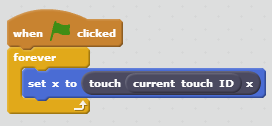
\includegraphics[width=0.4\textwidth]{images/OnePlayerPongAID.PNG}
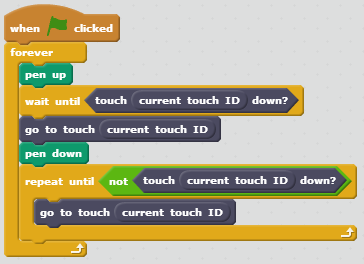
\includegraphics[width=0.59\textwidth]{images/OneFingerPaintingAID.PNG}
\caption[Sample Absolute Indexing Design Scripts for Low Floor Case Projects]{A sample Absolute Indexing Design script for the paddle controls in a one-player Pong game is on the left. On the right is a sample paintbrush script for one-finger painting.}
\label{LowFloorAID}
\end{figure}

By using the ``current touch ID" block to get the ID of the latest touch, both of the low floor case projects can be implemented in essentially the same way as was done using the previous two designs (Figure \ref{LowFloorAID}). Since we are assuming there is at most one touch on the screen at any time, the ``current touch ID" will always refer to the only touch on the tablet (if there is one).

Although these implementations look nearly as simple as those done with the Closest Finger Design, it might not be obvious to novice Scratchers that they can get access to the latest touch by inserting the ``current touch ID" block into the other touch blocks' (\emph{ID}) parameters. Blocks like ``touch (\emph{ID}) x" by themselves are neither tinkerable nor explorable, so it is difficult for Scratchers to learn how to use them without outside instruction. Unless the given (\emph{ID}) value happens to be an ID of one of the current touches, many of the Absolute Indexing Design blocks will appear unresponsive to touches.

One idea, to make the Absolute Indexing Design more explorable, would be for the block palette to feature  ``touch (\emph{ID}) x" and ``touch (\emph{ID}) y" blocks with the ``current touch ID" block already inserted in their (\emph{ID}) parameter. While this would definitely increase the explorability of the blocks, it could cause some confusion, because preassembled blocks have never before been featured in Scratch.


\subsection{Middle Height}

Once Scratchers get over the barrier of learning the intuition behind the  absolute indexing logic, they can, without too much difficulty, figure out how to implement both of the middle height case projects.

\begin{figure}
\centering
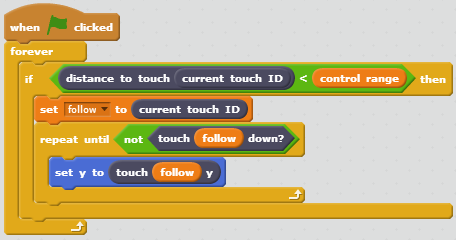
\includegraphics{images/BasicTwoPlayerPongAID.PNG}
\caption[Sample Absolute Indexing Design Script for Basic Two-Player Pong]
{Here is a sample script for controlling the paddle in a basic two-player Pong game using the Absolute Indexing Design.}
\label{BasicTwoPlayerPongAID}
\end{figure}

To begin, the controls for the basic two-player Pong game can be implemented by having both paddles constantly repeating a simple process (Figure \ref{BasicTwoPlayerPongAID}). First, each paddle's script can check to see if the touch with the ``current touch ID" is within their paddle's control range and store the ID in a variable if it is. Then, with the stored touch ID, the script can set the paddle to follow the touch with the stored ID until it is lifted.

Although this implementation of the basic two-player Pong game is complicated by the necessary use of a variable, experienced Scratchers generally have a basic understanding of how to use variables. As a result, barring the difficulty of understanding how the absolute indexing works, the complexity of this implementation is appropriate for a middle height project.

Like the basic two-player Pong game, the two-finger painting project can also be implemented using the Absolute Indexing Design by programming both of the paintbrushes to forever repeat a simple process while keeping a variable in which they store the ID of the touch they currently are following (Figure \ref{TwoFingerPaintingAID}). To begin each iteration of the repeated process, each paintbrush first checks to see if the touch with the ``current touch ID" is down and not being followed by the other paintbrush. If both criteria are met, then the paintbrush sets its variable to the current touch ID (thus claiming it) and follows the touch with its pen down until the touch is lifted.

\begin{figure}
\centering
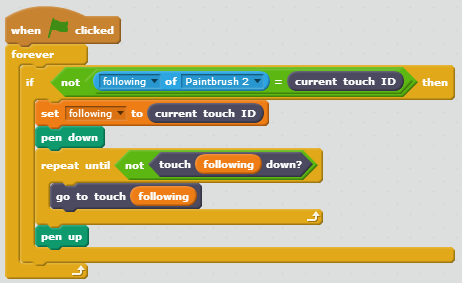
\includegraphics{images/TwoFingerPaintingAID.PNG}
\caption[Sample Absolute Indexing Design Script for Two-Finger Painting]
{Here is a sample script for controlling one of the paintbrushes in a two-finger painting project using the Absolute Indexing Design.}
\label{TwoFingerPaintingAID}
\end{figure}

Note that this implementation does rely on some of the specifics regarding Scratch's thread-switching protocol. However, the naive assumption that there will not be any race conditions in this case turns out to be true. As a result, this implementation is not too complicated for a middle height project. It is particularly noteworthy that two-finger painting can be implemented perfectly using the Absolute Indexing Design with an implementation that is no more complex as the imperfect implementations that could be created using the other two designs.

\subsection{High Ceiling}

When using the Absolute Indexing Design, the gap in complexity between the middle height and high ceiling case projects disappears. Once Scratchers have gained an intuition for how to use the Absolute Indexing Design to make multi-touch interactions with moderate complexity (which, granted, can be an arduous task), it becomes a natural and iterative process for them to discover how to make more complex ones.

\begin{figure}
\centering
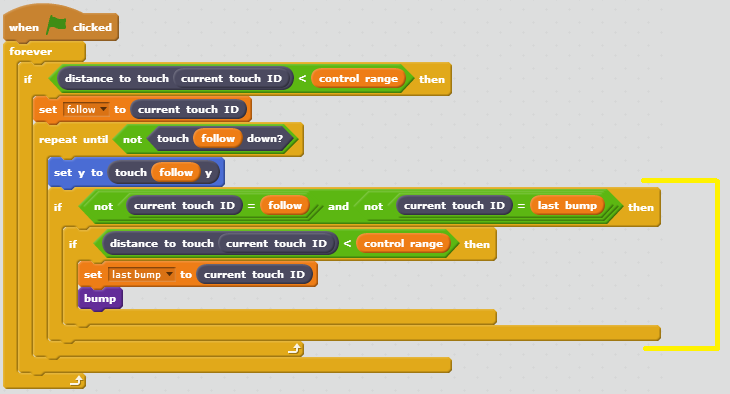
\includegraphics[width=0.8\textwidth]{images/AdvancedTwoPlayerPongAID.PNG}
\caption[Sample Absolute Indexing Design Script for Advanced Two-Player Pong]{Here is a sample script for controlling the paddle in an advanced two-player Pong game using the Absolute Indexing Design. The subroutine that is added to the basic two-player Pong game is highlighted. }
\label{AdvancedTwoPlayerPongAID}
\end{figure}

For example, the progression from the basic two-player Pong game to the advanced two-player Pong game is a particularly natural one when using the Absolute Indexing Design. To add the new bump interaction, each paddle's script can be augmented with an additional variable and a simple subroutine to be run when the paddle is following a particular touch (Figure \ref{AdvancedTwoPlayerPongAID}). The additional variable is used to store the ID of the touch that triggered the last bump, so that the same touch cannot trigger multiple bumps. Thus, the subroutine just checks on the current touch to see if it is different from both the touch the paddle is following and the touch that triggered the last bump. If both criteria are met, the subroutine makes a final check to see that the current touch is within the paddle's control range and initiates a bump if that is the case.

Similarly, the implementation for two-finger painting using the Absolute Indexing Design can easily be upgraded to ten-finger painting by simply adding more paintbrush sprites and more checks in each of their scripts to make sure that no paintbrush follows an already followed touch (Figure \ref{TediousMultiFingerPainting}). While this is an extremely simple augmentation, the script copying can become tedious. 

\begin{figure}
\centering
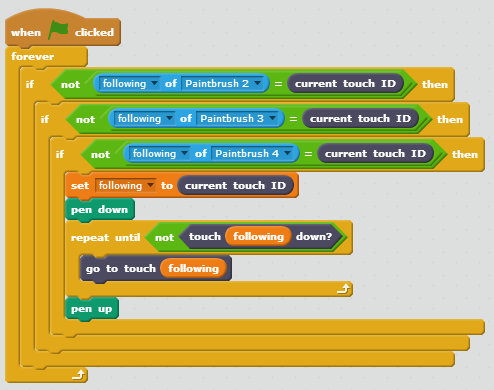
\includegraphics[width=0.6\textwidth]{images/TediousMultiFingerPainting.PNG}
\caption[Sample Absolute Indexing Design Script for Multi-Finger Painting]
{Here is a sample script for a paintbrush sprite in a four-finger painting project using the Absolute Indexing Design, but without using clones. To add more fingers, one need only add the additional paintbrush sprites and if statements.}
\label{TediousMultiFingerPainting}
\end{figure}

Hence, an experienced Scratcher may be tempted to use Scratch's cloning feature to make the implementation more elegant. Using the ``when touch created" block, a Scratcher can create a new paintbrush clone specifically to follow each new touch. The paintbrush clone would then follow its assigned touch until the touch is lifted, at which point the clone selflessly kills its own script to preserve computational resources. While the implementation using cloning is more elegant and uses fewer blocks, both implementations have the same functionality.

In comparison to the other two designs I have presented, the Absolute Indexing Design has a steep learning curve. It is very unlikely that someone could quickly figure out how the design's blocks work just by playing around with them. However, as multi-touch interactions become more complex, it becomes easier to implement them using the Absolute Indexing Design than with the other two designs.  


\chapter{Conclusion}

In this final chapter, I will begin by summarizing my analysis of the presented multi-touch interaction set designs presented and conclude by making suggestions for how this research may be furthered.

\section{Closing Remarks}

Even though each of the three multi-touch interaction set designs has its strengths, none of them fully satisfies the goals for maintaining low floors, wide walls, and high ceilings. While the minimalism of the Closest Finger Design  makes developing simple touch-interactivity accessible to beginners, it also precludes more advanced users from creating more complex interactions. In contrast, the Absolute Indexing Design is challenging for beginners to understand but, once understood, can be used to create limitlessly intricate multi-touch interactions. Meanwhile, the Relative Indexing Design sits uncomfortably in the middle, by being somewhat difficult to understand while still not being powerful enough to be used to implement even moderately complex multi-touch interactions.

Although I have presented these three multi-touch interaction set designs in isolation (in order to highlight their individual strengths and weaknesses), the best multi-touch interaction set is, arguably, most likely a combination of either two or all three of them. Ideally, Tablet Scratch's multi-touch interaction set will have the low floors of the Closest Finger Design and the high ceilings of the Absolute Indexing Design. However, it would be ill-advised to simply take the union of the two interaction set designs due to the confusion the considerable overlap would cause.

One way to combine the Closest Finger and Absolute Indexing designs would be to add both interaction sets to Tablet Scratch, but to feature them in separate locations. For example, Tablet Scratch could be designed so that sprites can only use the Closest Finger Design blocks and the stage can only use the Absolute Indexing Design blocks. This compromise is satisfactory on several levels. First, the closest finger is often not important for the stage in the same way that is for sprites. Furthermore, the Scratchers who assemble scripts for the stage are generally experienced and desire to make complex projects. Hence, only the Scratchers who need the more powerful blocks would be exposed to them.

While this combination preserves the Closest Finger Design's low floors, it does not quite preserve the Absolute Indexing Design's high ceilings. Since each sprite in this scenario can only access its closest touch, other touch information must be transferred from the stage to the sprite. Scratch does support such data transferring, but in certain scenarios it can be very difficult to implement robustly.

\section{Future Work}

Since low floors are generally achieved at the cost of high ceilings (and vice versa), it is unlikely that an indisputably ideal interaction set can ever be achieved. However, through more iteration and testing, we can get closer to designing a multi-touch interaction set that is perfect for the purposes of Tablet Scratch.

One important next step to reach this goal is to have the target audiences test the various multi-touch interaction set designs and then to iterate based on their experiences. Potential interaction set designs should each be tested with Scratchers of varying experience levels to ensure that the design makes implementing simple projects simple, and complex projects possible.

Although this thesis has focused on creating a multi-touch interaction set specifically within the context of Scratch, many of the ideas discussed are also applicable to designing touch-input-handling toolkits in general. There is little doubt that the toolkits used today in ``professional frameworks" are less than ideal. Not only do novice programmers have difficulty understanding how to use these toolkits, but even expert software engineers are prone to making errors while using them to develop multi-touch interactions. Despite the fact that virtually all commonly used multi-touch interactions have been developed with these professional frameworks, I am confident that it is possible to develop an equally functional multi-touch toolkit that is both more accessible and less vulnerable to bugs.


%% This defines the bibliography file (main.bib) and the bibliography style.
%% If you want to create a bibliography file by hand, change the contents of
%% this file to a `thebibliography' environment.  For more information 
%% see section 4.3 of the LaTeX manual.
\begin{singlespace}
\bibliography{main}
\bibliographystyle{unsrt}
\end{singlespace}

\end{document}

